\section{Kinematic Features}
Kinematic data structures in DART are designed to be comprehensive, extensible, and efficient for dynamic computation. Our design principles are heavily influenced by practical use cases suggested by researchers and practitioners in Robotics. We also follow the guidelines proposed by OSRF to make DART compatible with Gazebo standard.

\subsection{Skeleton, BodyNode, and Joint}
\begin{figure*}
\centering
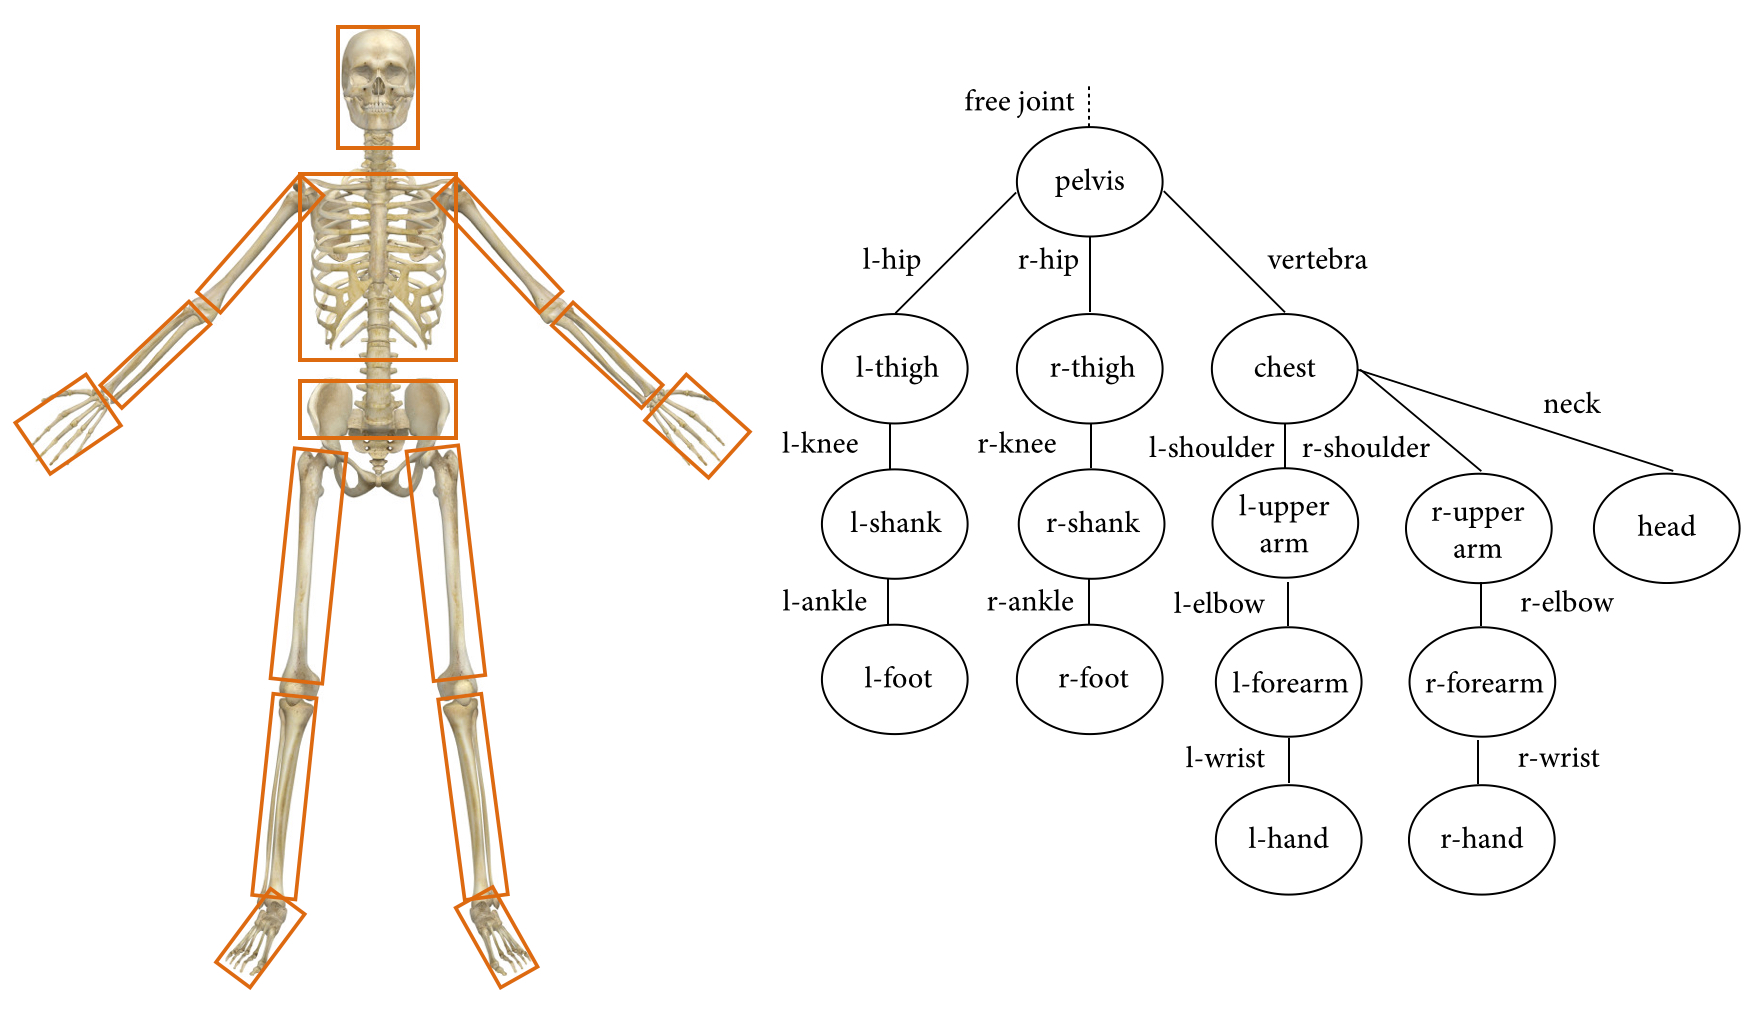
\includegraphics[width=6.0in]{skeletonTree.jpg}
\caption{Tasks for each research aim.}
\label{fig:skeleton}
\end{figure*}
 In DART, an articulated dynamics model is represented by a \textbf{Skeleton}. A Skeleton is a tree structure that consists of \textbf{BodyNode}s which are connected by \textbf{Joint}s. Every Joint has a child BodyNode, and every BodyNode has a parent Joint. Even the root BodyNode has a Joint that attaches it to the \textbf{World}. For example, the human skeleton can be organized into a tree structure (Figure \ref{fig:skeleton}) with nodes representing BodyNodes and edges representing Joints. Depending on the joint type (Section \ref{sec:jointTypes}), each joint has a specific number of degrees of freedom (DOFs). For example, the hip joint can be modeled by an \textbf{EulerJoint} with three DOFs, while a knee joint can be modeled by a \textbf{RevoluteJoint} with one DOF. In this model, we select the pelvis to be the root BodyNode, which connects to the World via a \textbf{FreeJoint} with six DOFs.

A kinematic chain is a sequence of transformations from one BodyNode to another in the Skeleton. Figure \ref{fig:parentChild}(a) illustrates the transformations between two intermediate BodyNodes denoted as Parent and Child. The coordinate frames of Parent, Child, and the joint between them are shown as the RGB arrows. Let $\vc{T}_{pj}$ be the transformation from the Parent frame to the joint frame and $\vc{T}_{cj}$ be the transformation from the Child frame to the joint frame. These two transformations are fixed and can be customized as part of the \textbf{Joint::Properties} of the joint. The transformation of the joint $\vc{T}(\vc{q})$ is a function of the DOFs, $\vc{q}$, associated with the joint. In the case of the hip joint, $\vc{q}$ is a 3x1 vector consisting of hip rotation angles in three dimensions. Thus, the transformation from the Parent frame to the Child frame is denoted by $\vc{T}_{pj}\vc{T}(\vc{q})\vc{T}_{cj}^T$.

\begin{figure*}
\centering
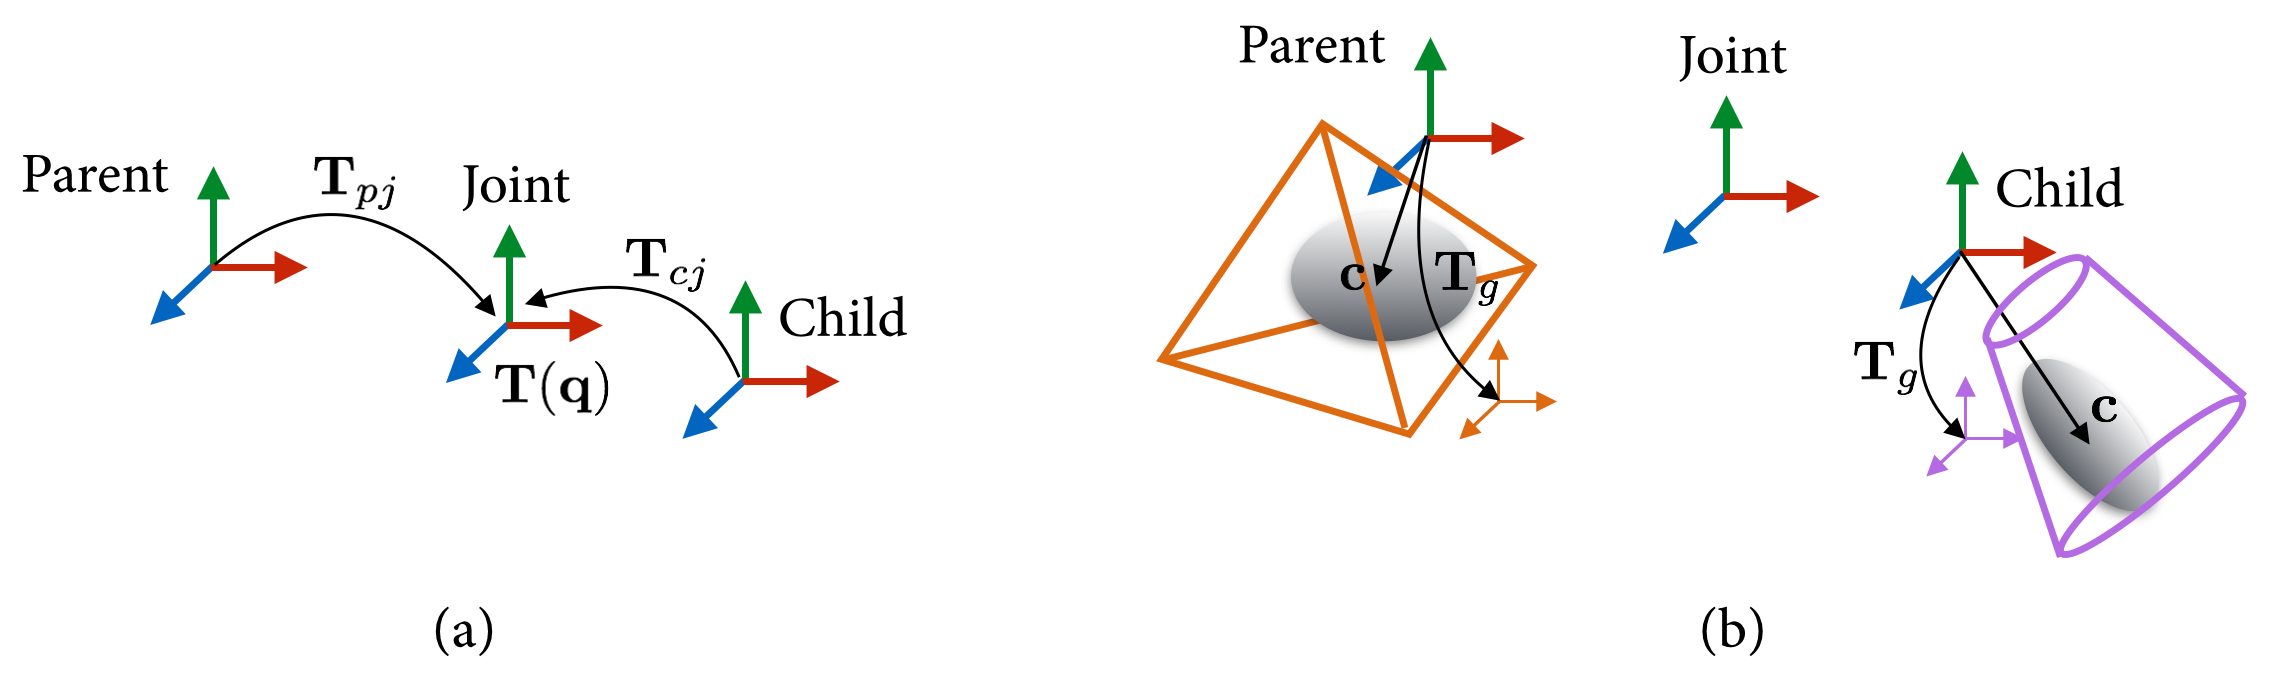
\includegraphics[width=6.0in]{parentChild.jpg}
\caption{Tasks for each research aim.}
\label{fig:parentChild}
\end{figure*}


\subsection{BodyNode Properties}
A BodyNode contains a set of customizable \textbf{BodyNode::Properties} to define its kinematic and dynamic behaviors.
\begin{itemize}[leftmargin=*] \itemsep1pt \parskip0pt \parsep0pt
  \item{\textbf{Inertial properties:}} The user can define the mass, the position of the center of mass in the BodyNode frame, and the moment of inertia around the center of mass in the BodyNode frame. The ellipsoids in Figure \ref{fig:parentChild}(b) illustrate the center of mass ($\vc{c}$) and the moment of inertia defined in the BodyNode frame.
  
\todo[MXG]{We should probably mention ShapeNode when discussing geometry}

  \item{\textbf{Geometry properties:}} The user can associate a set of \textbf{Shape}s with a BodyNode. Each shape has its own geometry information used by rendering and collision detection routines. DART supports a few primitive shapes, box, ellipsoid, cylinder, plane, line segment, in addition to arbitrary 3D polygons. Each shape can be defined in its own coordinate frame. The spatial relation between the Shape and its associated BodyNode is defined by a fixed transformation $\vc{T}_g$ (Figure \ref{fig:parentChild}(b)).
  \item{\textbf{Collision properties:}} The user can set the friction coefficient and the coefficient of restitution of a BodyNode, as well as the flag that determines whether the BodyNode is collidable.
\end{itemize}

\subsection{Joint types}
\label{sec:jointTypes}
DART supports 10 types of joints. Each joint type has a fixed number of DOFs and a specific configuration domain. Some joint types require the user to define their \textbf{UniqueProperties}. For example, the rotation axes of \textbf{RevoluteJoint}, \textbf{UniversalJoint} and \textbf{PlanarJoint} need to be specified when the joint is constructed. Likewise, the order of three axes (`xyz', `zyx', etc) in an \textbf{EulerJoint} needs to be predefined. These properties can be changed at any time, and the kinematics and dynamics calculations will automatically adjust to account for those changes. The only potential negative impact would be non-physical discontinuities if property changes are made during a simulation. Note that both \textbf{BallJoint} and \textbf{EulerJoint} are used to represent rotational motion in 3D space. However, a \textbf{BallJoint} is represented by an exponential map while an \textbf{EulerJoint} is represented by three consecutive 1D rotational matrices. All joint types provided by DART are listed in Table \ref{tab:jointTypes}.

\begin{table}[h]
\centering
\caption{Joint Types}
\begin{tabular}{|c|c|c|c|}
  \hline
  \textbf{Name} & \textbf{\#DOF} & \textbf{Configuration Domain}  & \textbf{Unique Properties}\\
  \hline
  BallJoint  &  3 & $SO(3)$  & \\
  \hline
  EulerJoint & 3  & $SO(2) \times SO(2) \times SO(2)$ & 3-axis order \\
  \hline
  FreeJoint  & 6 & $SE(3)$  &\\
  \hline
  PlanarJoint & 3  & $SE(2)$ & axis1 and axis2 \\
  \hline
  PrismaticJoint & 1  & $R$ & axis \\
  \hline
  RevoluteJoint & 1  & $SO(2)$ & axis \\
  \hline
  ScrewJoint & 1  & $SO(2)$ & axis and pitch \\
  \hline
  TranslationalJoint & 3  & $R^3$ &  \\
  \hline
  UniversalJoint & 2  & $SO(2) \times SO(2)$ & axis1 and axis2 \\
  \hline
  WeldJoint & 0  & $\emptyset$ &  \\
  \hline
\end{tabular}
\label{tab:jointTypes}
\end{table}

\subsection{Frame semantics}
Mathematical formulae are often expressed in terms of reference frames. This can make it difficult to directly program the formulae if your kinematic library is less expressive than the mathematical language. If a kinematic library only offers a frame's transformation with respect to its parent frame or the world frame, then you may need to repeatedly compute relative transformations between two arbitrary frames, which can easily introduce errors due to typos or confusion. Worse yet, the formulae for computing relative velocities and relative accelerations in non-inertial reference frames can be exceedingly complex and difficult to implement correctly. Take for example the equation to compute the relative linear acceleration of \textbf{Frame B} relative to \textbf{Frame A} in the coordinates of \textbf{Frame F}:

\begin{equation}
\label{eqn:rel_accel}
^{F}a_{BA} = ^{F}R_{O} ( ^{O}a_{B} - ^{O}a_{A} - ^{O}\dot{\omega}_{A} \times ^{O}p_{BA} - 2 ^{O}\omega_{BA} \times ^{O}v_{BA} - ^{O}\omega_A \times (^{O}\omega_{A} \times ^{O}p_{BA})
\end{equation}

Any small mistake, such as mixing up a plus with a minus or mixing up two of the variables, will produce potentially devastatingly incorrect results. Even the individual variables in the above expression each has a non-trivial formula to compute it, which must be implemented perfectly in order for any computations to come out correctly. These issues can pose considerable barriers to writing complex controller logic which is reliable enough to safely run on expensive robots.

KIDO addresses this issue by providing frame semantics. The forward kinematics of KIDO are handled by the underlying \textbf{Frame} class. The Frame class is a pure virtual class which provides the user with an interface to compute the kinematic values of a frame with respect to any other arbitrary frame. So instead of needing to implement equation \ref{eqn:rel_accel}, KIDO allows you to simply call the function:

\begin{lstlisting}
B->getLinearAcceleration(A,F);
\end{lstlisting}

Here are a few examples of what the Frame semantics API looks like:

\begin{lstlisting}
// Transformation Matrix
Eigen::Isometry3d Frame::getWorldTransform() const;
Eigen::Isometry3d Frame::getTransform(
    const Frame* withRespectTo = Frame::World()) const;

// Velocity
Eigen::Vector3d getLinearVelocity(
    const Frame* relativeTo = Frame::World(),
    const Frame* inCoordinatesOf = Frame::World()) const;
Eigen::Vector3d getAngularVelocity(
    const Frame* relativeTo = Frame::World(),
    const Frame* inCoordinatesOf = Frame::World()) const;
    
// Acceleration
Eigen::Vector3d getLinearAcceleration(
    const Frame* relativeTo = Frame::World(),
    const Frame* inCoordinatesOf = Frame::World()) const;
\end{lstlisting}

Note that an \textbf{Eigen::Isometry3d} is a specialized type of transformation matrix which exists in SE3.

Since \textbf{Frame} is a pure virtual interface class, we also need to have concrete implementations of it in order to perform forward kinematics. Most of the functions in \textbf{Frame} are actually implemented already; there are only five functions which derived classes need to implement:

\begin{lstlisting}
virtual const Eigen::Isometry3d& getRelativeTransform() const = 0;
virtual const Eigen::Vector6d& getRelativeSpatialVelocity() const = 0;
virtual const Eigen::Vector6d& getRelativeSpatialAcceleration() const = 0;
virtual const Eigen::Vector6d& getPrimaryRelativeAcceleration() const = 0;
virtual const Eigen::Vector6d& getPartialAcceleration() const = 0;
\end{lstlisting}

In the first three functions, the term \textit{Relative} means the quantity is relative to its parent frame. The first three functions are all that is needed to perform forward kinematics. The last two functions are used to reduce the number of computations when performing Featherstone's Articulated Body Algorithm for forward dynamics.

KIDO currently provides four concrete implementations of the \textbf{Frame} class:

\subsubsection{BodyNode Frame Implementation}

The \textbf{BodyNode} class is used to define the kinematic structure of a \textbf{Skeleton}. Because of this, it is very helpful for \textbf{BodyNode} to inherit the \textbf{Frame} class and be compatible with all of its forward kinematics and frame semantics features. The transformation, velocity, and acceleration of a \textbf{BodyNode} relative to its parent \textbf{Frame} is fully determined by its parent \textbf{Joint}. In the general case, it is not possible to explicitly move a \textbf{BodyNode} to an arbitrary transformation or give it an arbitrary velocity or acceleration. These physical quantities are all constrained by the parent \textbf{Joint} of the \textbf{BodyNode} as well as every \textbf{Joint} that it descends from. To achieve an arbitrary transformation for a \textbf{BodyNode}, KIDO offers an \textbf{InverseKinematics} module discussed later in this report \todo[MXG]{Link to InverseKinematics section}. KIDO does not currently offer an inverse differential kinematics module, but implementing one should be straightforward with the tools that KIDO does provide.

The BodyNode class and how to use it will be discussed in far greater detail throughout the rest of this report. In many ways, it is the cornerstone class of KIDO.

\subsubsection{SimpleFrame Implementation}

In some cases, it might be too cumbersome to be constrained by a \textbf{Joint} the way \textbf{BodyNode} is. If you want to have a reference \textbf{Frame} with a completely arbitrary transform, velocity, and acceleration, then being constrained by \textbf{Joint} can make things more difficult. Also, if you want your frame to represent a reference frame which is not a physical body, then the \textbf{BodyNode} class would be overkill.

For these reasons, we offer the \textbf{SimpleFrame} class. The \textbf{SimpleFrame} class is simply a Frame; it does not have any collision or inertial properties and therefore cannot be simulated. However, what \textbf{SimpleFrame} does offer is the ability to arbitrarily set its transformations, velocities, and accelerations. This can be done with the following functions:

\begin{lstlisting}
// Set transformation relative to parent Frame
void SimpleFrame::setRelativeTransform(const Eigen::Isometry3d& newRelTransform);

// Set transformation relative to any other Frame
void SimpleFrame::setTransform(
    const Eigen::Isometry3d& newTransform,
    const Frame* withRespectTo = Frame::World());
    
// Set the spatial velocity relative to the parent Frame, in the coordinates of this Frame
void SimpleFrame::setRelativeSpatialVelocity(
    const Eigen::Vector6d& newSpatialVelocity);
    
// Set the spatial velocity relative to the parent Frame, in the coordinates of any Frame
void SimpleFrame::setRelativeSpatialVelocity(
    const Eigen::Vector6d& newSpatialVelocity,
    const Frame* inCoordinatesOf);
    
// Set the spatial acceleration relative to the parent Frame, in the coordinates of this Frame
void SimpleFrame::setRelativeSpatialAcceleration(
    const Eigen::Vector6d& newSpatialAcceleration);

// Set the spatial acceleration relative to the parent Frame, in the coordinates of any Frame
void SimpleFrame::setRelativeSpatialAcceleration(
    const Eigen::Vector6d& newSpatialAcceleration,
    const Frame* inCoordinatesOf);
\end{lstlisting}

It is important to note that, by default, spatial quantities like spatial velocity and spatial acceleration should be given in the coordinates of the frame that they belong to (\textbf{not} in the coordinates of the parent frame). But KIDO does provide convenience functions that allow you to represent the spatial quantities in whichever coordinates you would like to. However, they still must represent the quantities \textbf{relative to} the parent, even if they're expressed in the coordinates of a different frame (i.e. the values are rotated).

For those who are not familiar or not comfortable with spatial quantities, KIDO also offers an API for classic 3D vectors, like those used in the traditional Newton-Euler equations of motion:

\begin{lstlisting}
void SimpleFrame::setClassicDerivatives(
    const Eigen::Vector3d& linearVelocity      = Eigen::Vector3d::Zero(),
    const Eigen::Vector3d& angularVelocity     = Eigen::Vector3d::Zero(),
    const Eigen::Vector3d& linearAcceleration  = Eigen::Vector3d::Zero(),
    const Eigen::Vector3d& angularAcceleration = Eigen::Vector3d::Zero());
\end{lstlisting}

Even though KIDO provides an API that supports both spatial and classic vectors, under the hood it only utilizes spatial vectors, because spatial vectors require fewer operations for forward differential kinematics. This also means that only spatial vectors get stored under the hood, and therefore if a user wants to set the velocity and/or acceleration using classic vectors, then all classic vectors must be provided simultaneously, or else the final result would depend on the order in which the classic vectors get set, which would be confusing and undesirable behavior.

\subsubsection{FixedFrame Implementation}

The \textbf{BodyNode} frame implementation is constrained by Joints while the \textbf{SimpleFrame} frame implementation is completely unconstrained. The \textbf{FixedFrame} implementation allows the user complete freedom in setting the initial relative transform, but after that it may not move. Its relative velocity and relative acceleration vectors are always exactly zero. \textbf{FixedFrame} instances do not even offer a way to change the relative transform after construction.

However, it is still possible for a class to inherit the \textbf{FixedFrame} class, and the inheriting class does have the authority to alter the relative transform. For example, the \textbf{EndEffector} class is a derivative of \textbf{FixedFrame} and allows the user to change the relative transform freely. But no matter how the relative transform gets changed, the relative velocity and relative acceleration will always be reported as zero, so altering a relative transform during a simulation could result in non-physical discontinuities.

\subsubsection{WorldFrame Implementation}

The \textbf{WorldFrame} is a very special case of the \textbf{Frame} class. It always returns identity for its relative transformation as well as its world transformation. Its velocities and accelerations are always zero. It is a singleton class which only gets created once per program, and every kinematic chain descends from it. To access the \textbf{WorldFrame}, simply call the function \textbf{Frame::World()}.

Conventional wisdom and good software engineering practices dictate that singletons should be avoided almost always. In the case of the \textbf{WorldFrame}, it is designed to be a read-only object whose values are never changed. Therefore it is not at risk of issues related to race conditions or unexpected interdependencies within the code.

\subsection{Kinematic state of the system}
DART provides a variety of ways to query the position and the velocity of the system in generalized, Cartesian, and spatial coordinates. 

\begin{lstlisting}
// Generalized coordinates
Eigen::VectorXd MetaSkeleton::getPositions() const;
Eigen::VectorXd MetaSkeleton::getVelocities() const;

// Cartesian coordinates
Eigen::Isometry3d Frame::getTransform(const Frame* _withRespectTo = Frame::World(), const Frame* _inCoordinatesOf = Frame::World()) const;
Eigen::Vector3d Frame::getLinearVelocity(const Eigen::Vector3d& _offset, const Frame* _relativeTo = Frame::World(), const Frame* _inCoordinatesOf = Frame::World()) const;
Eigen::Vector3d Frame::getAngularVelocity(const Frame* _relativeTo = Frame::World(), const Frame* _inCoordinatesOf = Frame::World()) const;
Eigen::Vector3d Skeleton::getCOM(const Frame* _withRespectTo = Frame::World()) const override;
Eigen::Vector3d Skeleton::getCOMLinearVelocity(const Frame* _relativeTo = Frame::World(), const Frame* _inCoordinatesOf = Frame::World()) const override;
Eigen::Vector3d BodyNode::getCOM(const Frame* _withRespectTo = Frame::World()) const;
Eigen::Vector3d BodyNode::getCOMLinearVelocity(const Frame* _relativeTo = Frame::World(), const Frame* _inCoordinatesOf = Frame::World()) const;

// Spatial coordinates
Eigen::Vector6d Frame::getSpatialVelocity(const Eigen::Vector3d& _offset, const Frame* _relativeTo, const Frame* _inCoordinatesOf) const;
\end{lstlisting}

For  example, if one wishes to know the transformation of the left
hand from the left upper arm expressed in the coordinate frame of the
pelvis, it can be achieved by 

\begin{lstlisting}
// Assume l-hand, l-upper-arm, and pelvis are pointers of BodyNode
 Isometry3d T = l-hand->getTransform(l-upper-arm, pelvis);
\end{lstlisting}

The velocity of any point in any BodyNode frame relative to any other
frame can be queried. For example, the relative linear velocity of a
local point, \emph{offset}, in the \emph{l-hand} frame from the origin of the \emph{l-upper-arm} frame expressed in the \emph{pelvis} frame can be accessed by

\begin{lstlisting}
 Vector3d v = l-hand->getLinearVelocity(offset, l-upper-arm, pelvis);
\end{lstlisting}


% \paragraph{Generalized coordinates.} The configuration of a skeleton can be accessed via the functions that return the generalized positions of a system.

% \begin{lstlisting}[caption=MetaSkeleton.h]
% // Get the positions for all generalized coordinates
% Eigen::VectorXd getPositions() const;

% // Get the positions for a subset of the generalized coordinates
% Eigen::VectorXd getPositions(const std::vector<size_t>& _indices) const;

% // Get the position of a single generalized coordinate
% double getPosition(size_t _index) const;

% // Get the velocities for all generalized coordinates
% Eigen::VectorXd getVelocities() const;

% // Get the velocities for a subset of the generalized coordinates
% Eigen::VectorXd getVelocities(const std::vector<size_t>& _indices) const;

% // Get the velocity of a single generalized coordinate
% double getVelocity(size_t _index) const;
% \end{lstlisting}

% \paragraph{Cartesian coordinates.}DART provides flexible API to query the transformation of a BodyNode relative expressed in any coordinate frame, with respect to any coordinate frame. 

% \begin{lstlisting}[caption=Frame.h]
% // Example: The transformation of the left hand from the left upper arm expressed in the coordinate frame of the pelvis can be accessed by 
% // Isometry3d T = l-hand->getTransform(l-upper-arm, pelvis);
% // , where l-hand, l-upper-arm, and pelvis are pointers of BodyNode.
 
% Eigen::Isometry3d getTransform(const Frame* _withRespectTo = Frame::World(), const Frame* _inCoordinatesOf = Frame::World()) const;
% \end{lstlisting}

% In the absence of the second and the third arguments, this function will return the transformation from the World to the BodyNode expressed in the World frame.

% In terms of Cartesian velocity, the linear velocity of any point in any BodyNode frame relative to any other frame can be queried. This linear velocity can be expressed in any coordinate frame. We can also query the angular velocity of a BodyNode relative to any other frame expressed in any frame.

% \begin{lstlisting}[caption=Frame.h]
% // Example: The relative linear velocity of a local point ''Vector3d offset(0.1, 0, 0)'' in the l-hand frame from the origin of the l-upper-arm frame expressed in the pelvis frame can be accessed by
% // Vector3d v = l-hand->getLinearVelocity(offset, l-upper-arm, pelvis);

% Eigen::Vector3d getLinearVelocity(const Eigen::Vector3d& _offset, const Frame* _relativeTo = Frame::World(), const Frame* _inCoordinatesOf = Frame::World()) const;

% Eigen::Vector3d getAngularVelocity(const Frame* _relativeTo = Frame::World(), const Frame* _inCoordinatesOf = Frame::World()) const;
% \end{lstlisting}

% DART also provides convenient API to access the state of the center of mass for a Skeleton.

% \begin{lstlisting}[caption=Skeleton.h]
% Eigen::Vector3d getCOM(const Frame* _withRespectTo = Frame::World()) const override;

% Eigen::Vector3d getCOMLinearVelocity(const Frame* _relativeTo = Frame::World(), const Frame* _inCoordinatesOf = Frame::World()) const override;
% \end{lstlisting}

% The same API is also provided for accessing the state of the center of mass for a BodyNode.

% \begin{lstlisting}[caption=BodyNode.h]
% Eigen::Vector3d getCOM(const Frame* _withRespectTo = Frame::World()) const;

% Eigen::Vector3d getCOMLinearVelocity(const Frame* _relativeTo = Frame::World(), const Frame* _inCoordinatesOf = Frame::World()) const;
% \end{lstlisting}

% \paragraph{Spatial coordinates.}

\subsection{Jacobian matrices}
Calculating Jacobian matrix is a common theme in forward simulation, inverse kinematics, and many other robotics or graphics applications. DART computes Jacobian matrices and its derivatives efficiently and provides API to access the results in various forms. 

\paragraph{Skeleton.} The full Jacobian matrix with respect to all DOFs in the system can be accessed via the member functions of Skeleton.

\begin{lstlisting}[caption=Skeleton.h]
math::LinearJacobian getLinearJacobian(const BodyNode* _bodyNode, const Eigen::Vector3d& _localOffset, const Frame* _inCoordinatesOf = Frame::World()) const override;

math::AngularJacobian getAngularJacobian(const BodyNode* _bodyNode, const Frame* _inCoordinatesOf = Frame::World()) const override;
\end{lstlisting}

The first function returns $J_v$ that maps the generalized velocity of
the system to the velocity of the point attached to \emph{bodyNode}
with an offset, \emph{localOffset}, from the origin of
\emph{bodyNode}, $\vc{v} = J_v \dot{\vc{q}}$. The second function
returns $J_{\omega}$ that maps the generalized velocity to the angular
velocity of \emph{bodyNode}, $\omega = J_{\omega}\dot{\vc{q}}$. The
last optional parameter, \emph{inCoordinatesOf}, determines in which
coordinate frame the Jacobian matrix is expressed. The full Jacobian
matrix that combines both $J_v$ and $J_{\omega}$ can be obtained by
the following function.

\begin{lstlisting}[caption=Skeleton.h]
math::Jacobian getJacobian(const BodyNode* bodyNode, const Eigen::Vector3d& localOffset, const Frame* inCoordinatesOf) const override;
\end{lstlisting}


% $R^T\frac{\partial T\vc{p}}{\partial \vc{q}} \in \vc{R}^{3\times n}$,
% where $R$ is the rotation part of the transformation from the World
% frame to the frame of \emph{inCoordinatesOf}, $T$ is the
% transformation from the World frame to the frame of \emph{BodyNode},
% $\vc{p}$ is a local coordinate indicated by \emph{localOffset} in the
% frame of \emph{bodyNode}, and $\vc{q}$ is the vector of DOFs of the
% system which has the size $n$. The second function returns 


% The submatrix containing the top three
% rows is the linear Jacobian matrix of the point attached to
% \emph{bodyNode} with an offset, \emph{localOffset}, from the origin of
% \emph{bodyNode}, while the submatrix containing the bottom three rows
% is the angular Jacobain matrix of the \emph{bodyNode} frame. The
% Jacobain matrix can be expressed in any coordinate frame specified by
% \emph{inCoordinatesOf}. If only linear or angular Jacobian matrix is
% needed, the following two functions can be used.


\paragraph{BodyNode.} More compact Jacobian matrices can be acquired
via the member functions of a BodyNode. Unlike the Jacobain matrices
for the entire Skeleton, these Jacobian matrices have $m$ columns, the number of DOFs on the kinematic chain from the root node to the BodyNode of interest.


\begin{lstlisting}[caption=BodyNode.h]
math::LinearJacobian getLinearJacobian(const Eigen::Vector3d& _offset, const Frame* _inCoordinatesOf = Frame::World()) const;

math::AngularJacobian getAngularJacobian(const Frame* _inCoordinatesOf = Frame::World()) const;

math::Jacobian getJacobian(const Eigen::Vector3d& _offset, const Frame* _inCoordinatesOf) const;
\end{lstlisting}

\paragraph{Joint.} Similar Jacobian functions are also available for
the Joint class. The number of columns of the Jacobian depends on the
number of DOFs of the joint. For example, a BallJoint returns a $6
\times 3$ Jacobian while a RevoluteJoint returns a $6 \times 1$ Jacobian.

\begin{lstlisting}[caption=Joint.h]
virtual math::Jacobian getLocalJacobian(const Eigen::VectorXd&
_positions) const = 0;
\end{lstlisting}



% Joint:
% /// Get generalized Jacobian from parent body node to child body node
%   /// w.r.t. local generalized coordinate
%   virtual const math::Jacobian getLocalJacobian() const = 0;

%   /// Get generalized Jacobian from parent body node to child body node
%   /// w.r.t. local generalized coordinate
%   virtual math::Jacobian getLocalJacobian(
%       const Eigen::VectorXd& _positions) const = 0;

%   /// Get time derivative of generalized Jacobian from parent body node
%   /// to child body node w.r.t. local generalized coordinate
%   virtual const math::Jacobian getLocalJacobianTimeDeriv() const = 0;

\subsection{Skeleton modeling}
Building a complex skeleton from scratch can be very
difficult and tedious. Often time, the developer may prefer to modify an
existing skeleton described by a URDF or SDF file. DART provides many
functions to facilitate skeleton editing summarized in the following
table.

\begin{table}[h]
\centering
\caption{Functions for Skeleton Modeling}
\begin{tabular}{|L{3.3in}|L{2.7in}|}
  \hline
  \textbf{Function Example} & \textbf{Description} \\
  \hline
  bd1-$>$\textbf{remove}() & Remove BodyNode bd1 and its subtree from their Skeleton.  \\
  \hline
   bd1-$>$\textbf{moveTo}(bd2) & Move BodyNode bd1 and its subtree under BodyNode bd2.  \\
  \hline
 auto newSkel = bd1-$>$\textbf{split}("new skeleton") & Remove BodyNode bd1 and its subtree from their current Skeleton and move them into a newly created Skeleton named "new skeleton".  \\
  \hline
 bd1-$>$\textbf{changeParentJointType}$<$BallJoint$>$() & Change the joint type of BodyNode bd1's parent joint to BallJoint.  \\
  \hline
bd1-$>$\textbf{copyTo}(bd2) & Create a clone of BodyNode bd1 and its subtree
                   and attach the clone to an existing BodyNode bd2. \\
  \hline
 auto newSkel = bd1-$>$\textbf{copyAs}("new skeleton") & Create a
                                                         clone of
                                                         BodyNode bd1
                                                         and its
                                                         subtree as a new skeleton named "new skeleton".  \\
  \hline
\end{tabular}
\label{tab:skeletonEdit}
\end{table}

Some functions have optional parameters for more advanced modeling
operations. For example, \textbf{moveTo} is templated by \textbf{JoinType} and
can take in \textbf{Joint::Properties} as an argument, such as:
bd1->moveTo<EulerJoint>(bd2, properties).

\subsection{Inverse kinematics}
\red{Grey}
